\subsection{Расчет координат восходящего знака (Asc)}

Наша планета вращается не только вокруг Солнца, но и вокруг своей оси, что является причиной смены дня и ночи. Для удобства измерения времени и пространства Земля разделена на 360 условных линий --- долгот. Полный оборот вокруг своей оси Земля делает за 24 часа, или 1440 минут. Если разделить 1440 минут на 360, мы получим 4 минуты --- время поворота Земли на \(1^\circ\), или время прохождения Солнца между долготами.

Восходящий знак --- это одно из созвездий Зодиака, которое появляется на восточном горизонте в момент рождения человека. Расчет координат восходящего знака --- это расчет координат точки эклиптики на восточном горизонте в момент рождения. Точка назвается \emph{асцедент} и обозначается в эфемеридах --- \emph{Asc}. Необходимо знать, что каждый знак Зодиака занимает \(30^\circ\) пространства. Всего в гороскопе 12 знаков: \(12 * 30^\circ = 360^\circ\) --- полный Зодиак.

Асцендент проходит через \(360^\circ\) полного Зодиака за 24 часа.

Теперь мы можем начать расчет асцендента на нашем примере. Вначале необходимо определить сидерическое(звездное) время в момент рождения человека. В эфемеридах оно указано для каждого дня в 0 часов по Гринвичу и обозначается \emph{Sid Time}.

Откроем эфемериды на странице, где указано сидерическое время для 4 и 5 декабря 1957 года, и выпишем его значения:

\begin{mylist}
	\item 4 декабря 1957 года Sid. Time = \timeshort{4}{50}{10}
	\item 5 декабря 1957 года Sid. Time = \timeshort{4}{54}{7}
\end{mylist}

Далее, решая пропорцию, определяем звездное время в момент рождения(\timeshort{9}{35}{}) по Гринвичу:

\calc{\dfrac{4:54:07 - 4:50:10}{24} * 9:35 + 4:50:10 = 4:51:44}

Теперь требуется определить географические координаты города Харькова. Еще раз возьмем известный нам справочник и на странице 32 найдем Харьков. Выпишем координаты, соответствующие месту нахождения города:

\begin{mylist}
	\item северная широта --- \coord{50}{00}{00}
	\item восточная долгота --- \coord{36}{15}{00}
\end{mylist}

Если нет справочника, определим географические координаты города Харькова по атласу.

Переведем долготу во время путем деления на 15. Это связано с тем, что скорость вращения Земли равна \(15^\circ\) долготы в час. Теперь у нас есть три величины времени:

\begin{mylist}
	\item время рождения --- \timeshort{9}{35}{}
	\item звездное время --- \timeshort{4}{51}{44}
	\item долготное время --- \timeshort{2}{25}{}
\end{mylist}

Так как Харьков находится в восточном полушарии, то сложим эти три величины времени:

\calc{9:35 + 4:51:44 + 2:25 = 16:51:44}

Полученный результат является окончательным звездным временем. Используя таблицы домов Плацидуса (или Коха) найдем звездную величину \timeshort{16}{51}{44} в графе \emph{Sid. Time}. В таблице домов величина \timeshort{16}{51}{44} находится между двух других величин звездного времени --- \timeshort{16}{50}{34} и \timeshort{16}{54}{53}. Напротив первого звездного времени на широте \(50^\circ\) в графе \emph{Asc} вы увидите данные \(23^\circ\)\aquarius\(23^\prime\) (напомним: \aquarius --- Водолей), а напротив другоо звездного времени на той же широте в графе \emph{Asc} будут другие данные: \(25^\circ\)\aquarius\(24^\prime\). В таблице домов Плацидуса это выглядит так:

 
\begin{table}[tph!]
	\centering

	% Расширить по вертикали
	\renewcommand{\arraystretch}{1.5}

	% Заполним данными
	\begin{tabular}{|c|c|c|c|}
		\hline
		\emph{Sid. Time}  & Lat \(49^\circ\) \emph{Asc} & Lat \(50^\circ\) \emph{Asc} & Lat \(51^\circ\) \emph{Asc} \\
		\hline
		\calc{16 - 50 - 34} & \(24^\circ\)\aquarius\(29^\prime\) & \(23^\circ\)\aquarius\(23^\prime\) & \(22^\circ\)\aquarius\(11^\prime\) \\
		\calc{16 - 54 - 53} & \(26^\circ\)\aquarius\(28^\prime\) & \(25^\circ\)\aquarius\(24^\prime\) & \(24^\circ\)\aquarius\(14^\prime\) \\
		\hline
	\end{tabular}
\end{table}

\begin{myenum}
	\item Определим разницу между двумя звездными величинами, указанными в таблице(в минутах):
		\calc{16:54:53 - 16:50:34 = 4:19:00 = 4.316}
	\item Определим разницу между окончательной звездной величной (\timeshort{16}{51}{44}) и первой звездной величиной, указанной в таблице (\timeshort{16}{50}{34})(в минутах):
		\calc{16:51:44 - 16:50:34 = 00:01:10 = 1.16}
	\item Определим разницу между двумя величинами, которые указаны в графе \emph{Asc} на широте \(50^\circ\) (Lat. \(\50^\circ\) (в минутах):
		\calc{\(25^\circ\)\aquarius\(24^\prime\) - \(23^\circ\)\aquarius\(23^\prime\) = \coord{2}{1}{0} = 2.016}
	\item Определим асцендент. \coord{23}{23}{00} можно записать как 23,383\(^\circ\):
		\calc{\dfrac{2.016}{4.316} * 1.16 + 23.383 = 23.924834} или \coord{23}{55}{29} Водолея
	\item Вычитаем величину уже известной нам аянамсы:
		\calc{\coord{23}{55}{29} - \coord{23}{16}{21} = \coord{00}{39}{08}}
\end{myenum}

Итак, асцендент равен \coord{00}{39}{08} Водолея. На этом заканчивается расчет карты рождения в нашем гороскопе-примере.

В момент рождения человека (4 декабря 1957 года в \timeshort{12}{35}{} по местному времени) планеты и восходящий знак имели следующие координаты:

\begin{table}[tph!]
	\centering

	% Расширить по вертикали
	\renewcommand{\arraystretch}{1.5}

	% Заполним данными
	\begin{tabular}{|ll|}
		\hline
		Асцендент & \coord{00}{39}{08} Водолея \\
		Солнце   & \coord{18}{42}{36} Скорпиона \\
		Луна     & \coord{14}{51}{12} Овна \\
		Марс     & \coord{23}{56}{00} Весов \\
		Меркурий & \coord{09}{09}{00} Стрельца \\
		Юпитер   & \coord{01}{03}{00} Весов \\
		Венера   & \coord{04}{48}{00} Козерога \\
		Сатурн   & \coord{22}{56}{00} Скорпиона \\
		Раху     & \coord{17}{03}{00} Весов \\
		Кету     & \coord{17}{03}{00} Овна \\ \hline
	\end{tabular}
\end{table}

Перечисленные координаты планет и асцендента определяют картину звездного неба в момент рождения человека. Она будет индивидуальна для каждого и никогда ни для кого другого не повторится. Звездная картина как бы накладывает особую печать на характер, поведение, наклонности и судьбу человека. Для удобства её прочтения мы должны расположить асцендент и планеты в соответствии с их координатами в специальной диаграмме.

В практике астрологов применяются различные виды диаграмм. Например:
\newline

{\parindent=0
	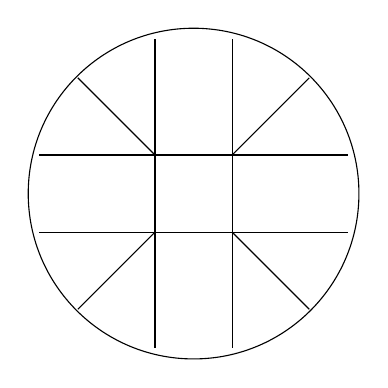
\begin{tikzpicture}[scale=0.7]
		\draw (-2.8,0.7) -- (2.8,0.7);
		\draw (-2.8,-0.7) -- (2.8,-0.7);
		\draw (0.7,-2.8) -- (0.7,2.8);
		\draw (-0.7,-2.8) -- (-0.7,2.8);
		\draw (-2.1,2.1) -- (-0.7,0.7);
		\draw (-2.1,-2.1) -- (-0.7,-0.7);
		\draw (0.7,0.7) -- (2.1,2.1);
		\draw (0.7,-0.7) -- (2.1,-2.1);
		\draw (0,0) circle(3);
	\end{tikzpicture}
	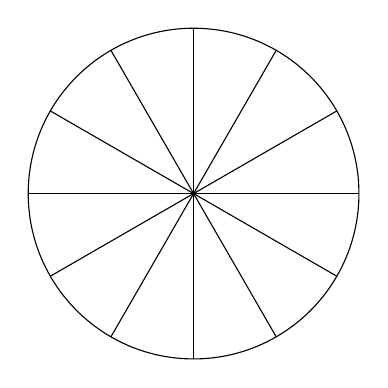
\begin{tikzpicture}[scale=0.7]
		\draw (-3,0) -- (3,0);
		\draw (-3,0) -- (3,0);
		\draw (0,-3) -- (0,2.8);
		\draw (0,-3) -- (0,3);
		\draw (-2.6,-1.5) -- (2.6,1.5);
		\draw (-1.5,-2.6) -- (1.5,2.6);
		\draw (-2.6,1.5) -- (2.6,-1.5);
		\draw (-1.5,2.6) -- (1.5,-2.6);
		\draw (0,0) circle(3);
	\end{tikzpicture}
	\begin{tikzpicture}[scale=0.7]
		\draw (-3,3) -- (3,3);
		\draw (-3,-3) -- (3,-3);
		\draw (-3,-3) -- (-3,3);
		\draw (3,-3) -- (3,3);
		\draw (-1.5,-3) -- (-1.5,3);
		\draw (1.5,-3) -- (1.5,3);
		\draw (-3,-1.5) -- (3,-1.5);
		\draw (-3,1.5) -- (3,1.5);
		\draw (0,-3) -- (0,-1.5);
		\draw (0,1.5) -- (0,3);
		\draw (-3,0) -- (-1.5,0);
		\draw (1.5,0) -- (3,0);
	\end{tikzpicture}
	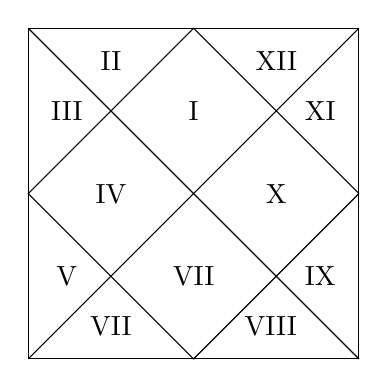
\begin{tikzpicture}[scale=0.7]
		\draw (-3,3) -- (3,3);
		\draw (-3,-3) -- (3,-3);
		\draw (-3,-3) -- (-3,3);
		\draw (3,-3) -- (3,3);
		\draw (-3,-3) -- (3,3);
		\draw (-3,3) -- (3,-3);
		\draw (3,0) -- (0,-3) -- (-3,0) -- (0,3) -- (3,0);

		% подписи
		\draw (-1.5,2.4) node{II};
		\draw (1.5,2.4) node{XII};

		\draw (-2.3,1.5) node{III};
		\draw (0,1.5) node{I};
		\draw (2.3,1.5) node{XI};

		\draw (-1.5,0) node{IV};
		\draw (1.5,0) node{X};

		\draw (-2.3,-1.5) node{V};
		\draw (0,-1.5) node{VII};
		\draw (2.3,-1.5) node{IX};

		\draw (-1.5,-2.4) node{VII};
		\draw (1.4,-2.4) node{VIII};
	\end{tikzpicture}
}

В нашей книге мы будем использовать диаграмму, показанную в последнем примере, которая наиболее популярна в индийской астрологии. Каждый ее сектор представляет дом, который имеет свой номер. Функциональный порядок расположения домов указан на диаграмме от одного до двеннадцати. Он никогда не изменяется, поэтому номера домов в диаграмме цифрами не обозначаются. Цифрами обозначены только знаки Зодиака согласно их порядковому номеру. Знаки зодиака идут в определенной последовательности и имеют свои порядковые номера:


\begin{table}[tph!]
	\centering

	% Расширить по вертикали
	\renewcommand{\arraystretch}{1.5}

	% Заполним данными
	\begin{tabular}{lll}
		1 --- Овен     & 5 --- Лев      & 9 --- Стрелец \\
		2 --- Телец    & 6 --- Дева     & 10 --- Козерог \\
		3 --- Близнецы & 7 --- Весы     & 11 --- Водолей \\
		4 --- Рак      & 8 --- Скорпион & 12 --- Рыбы \\
	\end{tabular}
\end{table}

Так как каждому знаку соответствует определенный номер, то вместо символических обозначений мы будем использовать в диаграмме соответствующие цифры.

В нашем примере восходящим знаком является Водолей, и его номерной знак --- это всегда первый (I) дом, поэтому в секторе, который соответствует первому дому, поставим цифру 11. Во втором (II) доме --- цифру 12, в третьем (III) доме --- цифру 1, в четвертом (IV) доме --- цифру 2, в пятом (V) доме --- цифру 3, в  шестом (VI) доме --- цифру 4, в седьмом (VII) доме --- цифру 5, в восьмом (VIII) доме --- цифру 6, в девятом (IX) доме --- цифру 7, в десятом (X) доме --- цифру 8, в одиннадцатом (XI) доме --- цифру 9 и в двеннадцатом (XII) доме --- цифру 10. Теперь поместим уже расчитанные планеты в сектора, соответствующие номерам знаков Зодиака. В диаграмме это будет выглядеть так:

\natal[asc=11,three=Луна\\Кету,nine=Раху\\Юпитер\\Марс,ten=Солнце\\Сатурн,eleven=Меркурий,twelve=Венера]{}

Это и есть карта рождения, составленная по индийской астрологической системе. Определим, в каких домах находятся планеты:

\begin{mylist}
	\item Луна и Кету --- в 3-м доме.
	\item Юпитер, Раху и Марс --- в 9-м доме.
	\item Солнце и Сатурн --- в 10-м доме.
	\item Меркурий --- в 11-м доме.
	\item Венера --- в 12-м доме.
\end{mylist}

Что означают позиции планет в различных домах, вы узнаете в следующих главах книги.

Индийская астрология --- предсказательная астрология, поэтому вы должны научиться расчитывать периоды жизни, которые связаны с расчетами главных периодов и подпериодов планет.
